\section{Practical Aspects}

We address here some issues that arise when implementing the described algorithm on a resource-constrained platform. Furthermore, many practical expedients allow to deal with limited sampling budget, slow control rates and finally with sim-to-real transfer.  

\subsection{Gradient Clipping} 
The policy update rule in \eqn \ref{eq:update_rule} consists is a recedigin horizon \emph{mini-batch} SGD. As a consequence, the gradient variance can greatly vary between successive iteration of the algorithm. To prevent this phenomenon, especially evident with small sampling budget, we clip the gradients to a user-defined threshold.  

\subsection{Receding Horizon Control} 
Model-based predictive control rarely achieves the rate of common low-level controllers (around 100Hz or higher depending on the system) because of the intensive optimization performed at every iteration step. Nevertheless, the predicted horizon can be used in open loop by a cascaded trajectory tracking controller before the new optimization step has completed. Therefore the stochastic controller keeps an internal copy of the previously optimized trajectory. Then, the low-level controller executes in open loop the input sequence. The sequence is swapped by the controller once a new one is available.

At the beginning of a new optimization all the stored rollouts are shifted back by the real-time number of steps elapsed since the last optimization. A subset of the best rollouts (assuming they are ordered) are kept to warm start the next iteration. For these, the actual deviation from the optimal input needs to be recomputed.

The solutions provided by the sampling-based controller are not sufficiently smooth for a practical application, especially with a big step size and no momentum. 
In order to filter the solution without introducing additional delays, we apply a moving window Savitzky-Golay filter~\cite{gorry1990general}. 

\subsection{Adaptive temperature} 
The coefficient $\lambda$ in \eqref{eq:update_rule} determines how ``aggressive" the weighting is between different trajectories. Adopting a constant value would give a numerically zero weight to most of the trajectories. Shifting the trajectory cost by the minimum cost as proposed in~\cite{williams_information_2017} also does not alleviate this issue. 
Especially in regions of high cost, trajectories that are equivalently good can be assigned very different weights. We instead propose to adopt the same technique as in~\cite{theodorou2010generalized} where the parameter $\lambda$ can be automatically optimized to maximally discriminate between the experienced trajectories. The modified exponential utility is then defined by,
\begin{equation} \label{eq:adaptive_t}
    \exp (-\lambda J ) = \exp \left( -h \frac{J - J_{\min}}{J_{\max} - J_{\min}} \right).
\end{equation}
\add{Need to show average reward with and without adaptive temperature}

\subsection{Simulator Tuning}
A first but rather important set of tuning parameters are the simulation controller gains. 
It is advisable to set  low gains in order to keep the whole system stable during rollouts and avoid high interaction forces that might arise during contact. This in turn also reduces the low-level controller bandwidth which behaves as a low-pass filter for the reference velocities, which are often non-smooth due to the random sampling. Crucial to the overall performance is the fidelity of the simulation environment (implementing \eqn \ref{eq:eom}). Unfortunately the discrepancy between the simulator and the real physical model known as \emph{sim-to-real} gap is always present. A typical failure case consists in a over-estimation of objects friction. We have experienced that in these cases the controller would try to manipulate the object by ``scratching" its surface with the finger tip. This approach could be immediately related to the fact that the simulator assumed a high friction coefficient between the two materials. In practice friction is hard to measure and depends on the contact patch between surfaces. This is extremely challenging to transfer from simulation to hardware. Instead kinematic constraints between contact points depends on the system geometry which can be accurately measured (e.g from CAD models). Therefore solutions that exploit the latter are more likely to succeed on the real platform. One can bias the controller towards these solutions by setting, for example, a very low friction coefficient between contact bodies.

\subsection{Contact-meshes simplification}
A large proportion of simulation time is spent on collision detection. We reduce the component meshes to the relevant ones and simplify to primitive shapes, as shown in \fig\ref{fig:1}. We are especially interested in the collision objects belonging to the robot end-effector and the object. This adaptation tremendously reduces computation especially during the contact phase. The original collision mesh, besides being inaccurate, slows down collision checking. A simplified yet accurate model consisting of primitive shapes produces a significant speed-up as we can see in \fig\ref{fig:rate_comparison}. Some additional statistics are also presented in Table~\ref{tab:rate_stat}.

\begin{figure}[t]
\centering
\hfill
\begin{subfigure}{0.3\columnwidth}
    \includegraphics[width=\linewidth]{figures/hardware/m mesh_cropped.pdf}
    \caption{}
\end{subfigure}%
\hfill
\begin{subfigure}{0.3\columnwidth}
    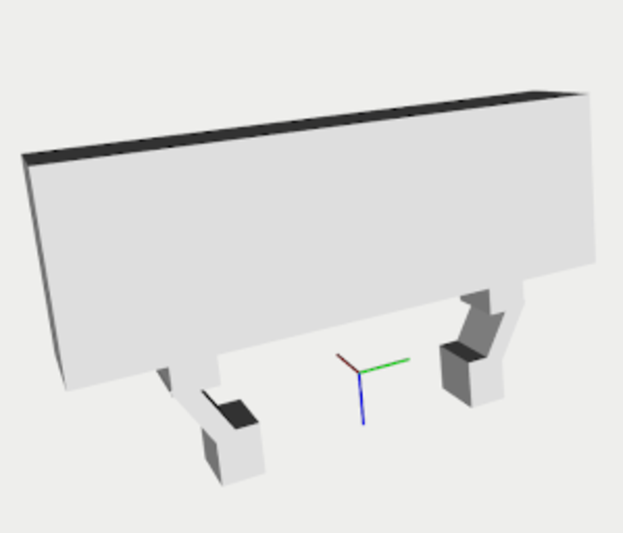
\includegraphics[width=\linewidth]{figures/doulbe_simple_cropped.pdf}
    \caption{}
\end{subfigure}%
\hfill
\begin{subfigure}{0.3\columnwidth}
    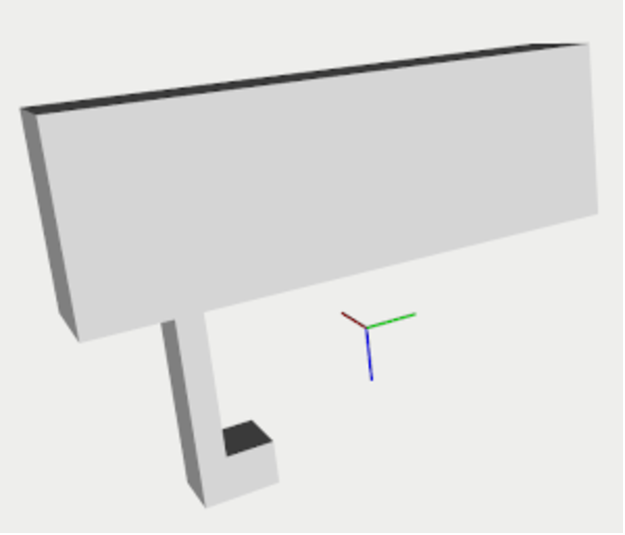
\includegraphics[width=\linewidth]{figures/single_hook_cropped.pdf}
    \caption{}
\end{subfigure}
\hfill
\caption{This figure shows three different collision shapes for the robot end-effector: (a) original mesh, (b) simplified collision shape, (c) modified hook design. Original collision meshes are often approximated by convex hulls which are inaccurate and more complex representations.}\label{fig:1}
\end{figure}


\begin{table}[h!]
    \centering
    \begin{tabular}{c|c|c|c}
             &  Min Rate [Hz] & Max Rate [Hz]& Average Rate[Hz]\\
                       \hline
         Original mesh & 10 & 306 & 145 \\
         Two fingers & \textbf{49} & 321 & 161 \\
         Hook finger & 44 & \textbf{327} & \textbf{177} \\
    \end{tabular}
    \caption{Control rate statistics when using different collision shapes for the door opening task.TODO: update with new values}
    \label{tab:rate_stat}
\end{table}

 
\subsection{Cascaded control architecture}
The expensive rollouts sampling procedure often limits the rate of the controller. Instead, the QP can be efficiently solved at almost the same rate as the low level controller. We propose a \emph{cascaded control} architecture composed of a low rate sampling and policy verification block and a high rate low level control loop. The latter reuses the QP previously defined to find the best input according to the latest received measurements. 
\begin{figure}[t!]
\centering
\hspace*{-1.0cm}
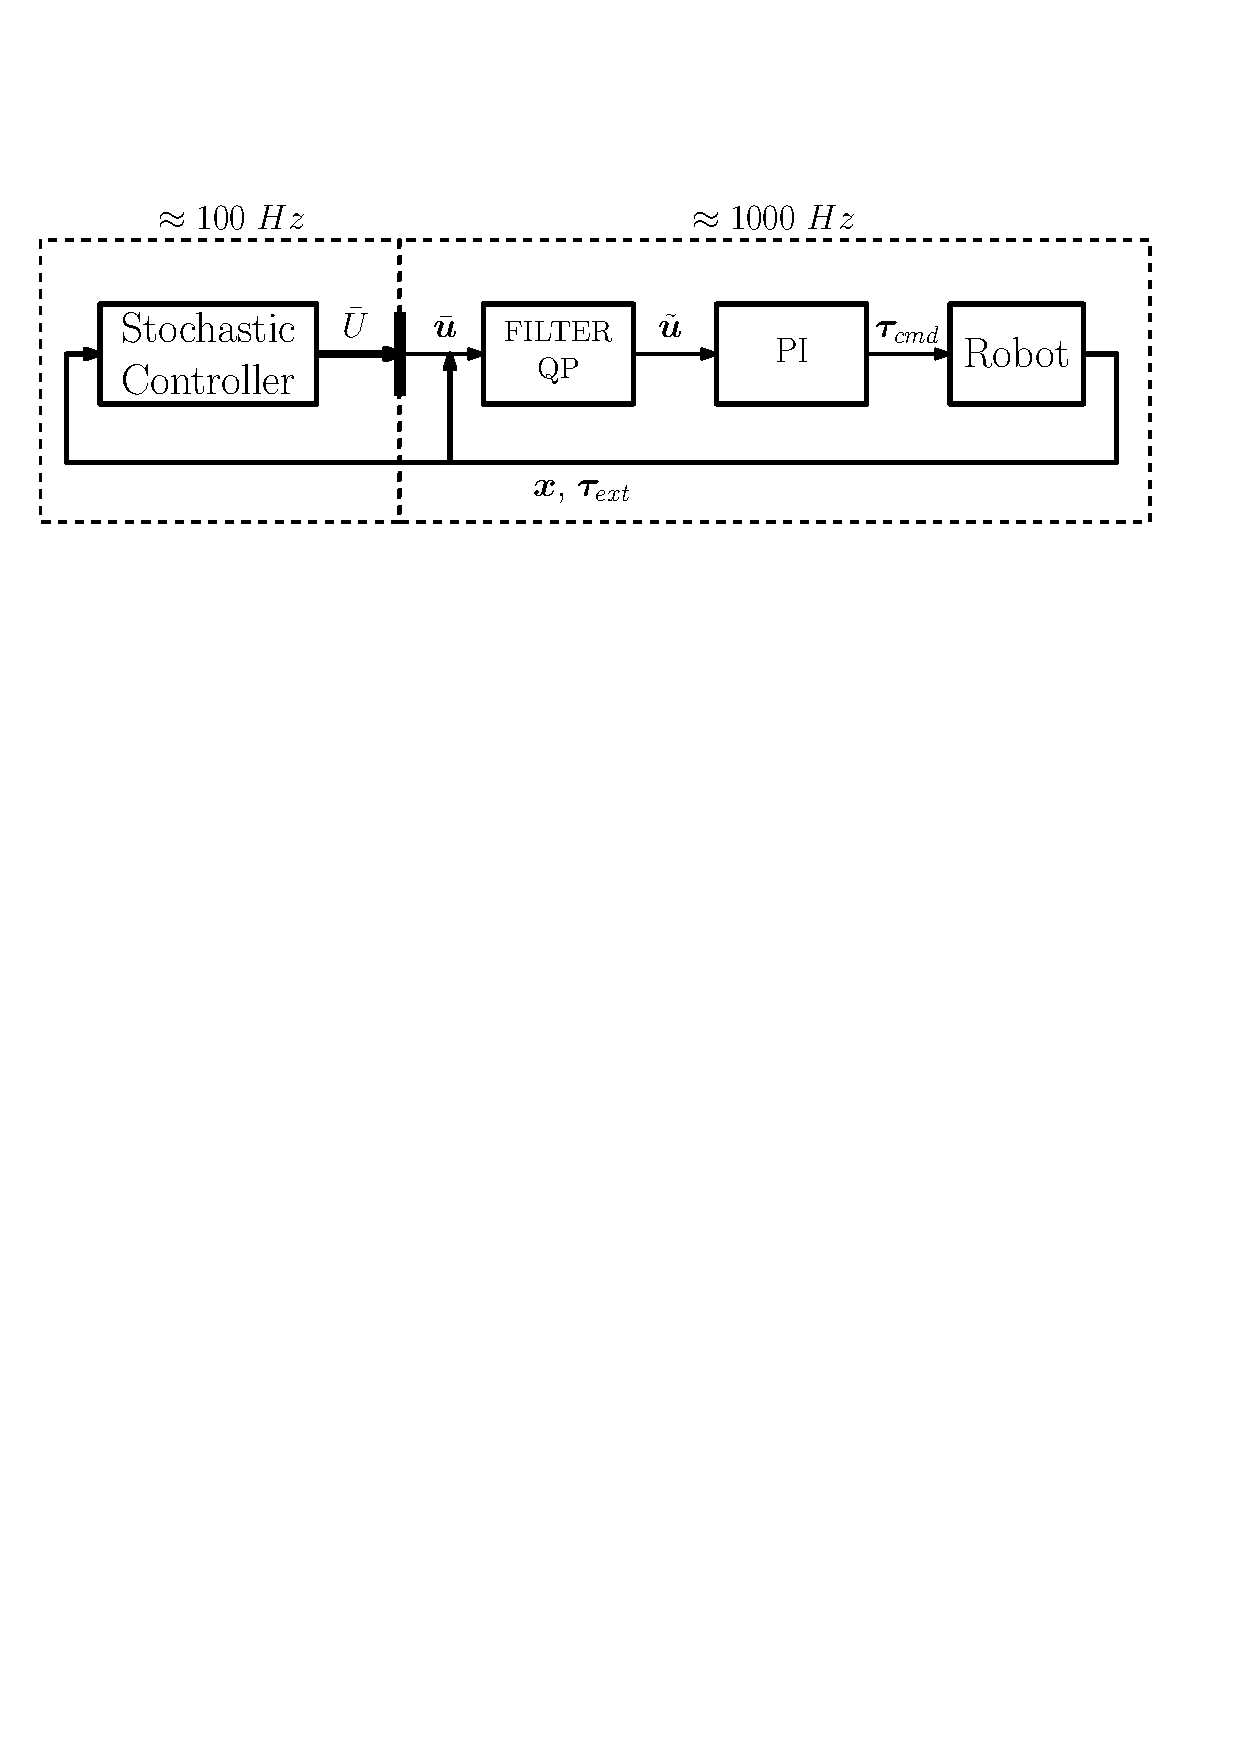
\includegraphics[width=1.1\columnwidth]{figures/schemes/high_level_architecture.pdf}
\caption{Put caption cascaded control architecture} \label{fig:cascaded_architecture}
\end{figure}

\begin{figure}[t!]
\centering
\hspace*{-1.0cm}
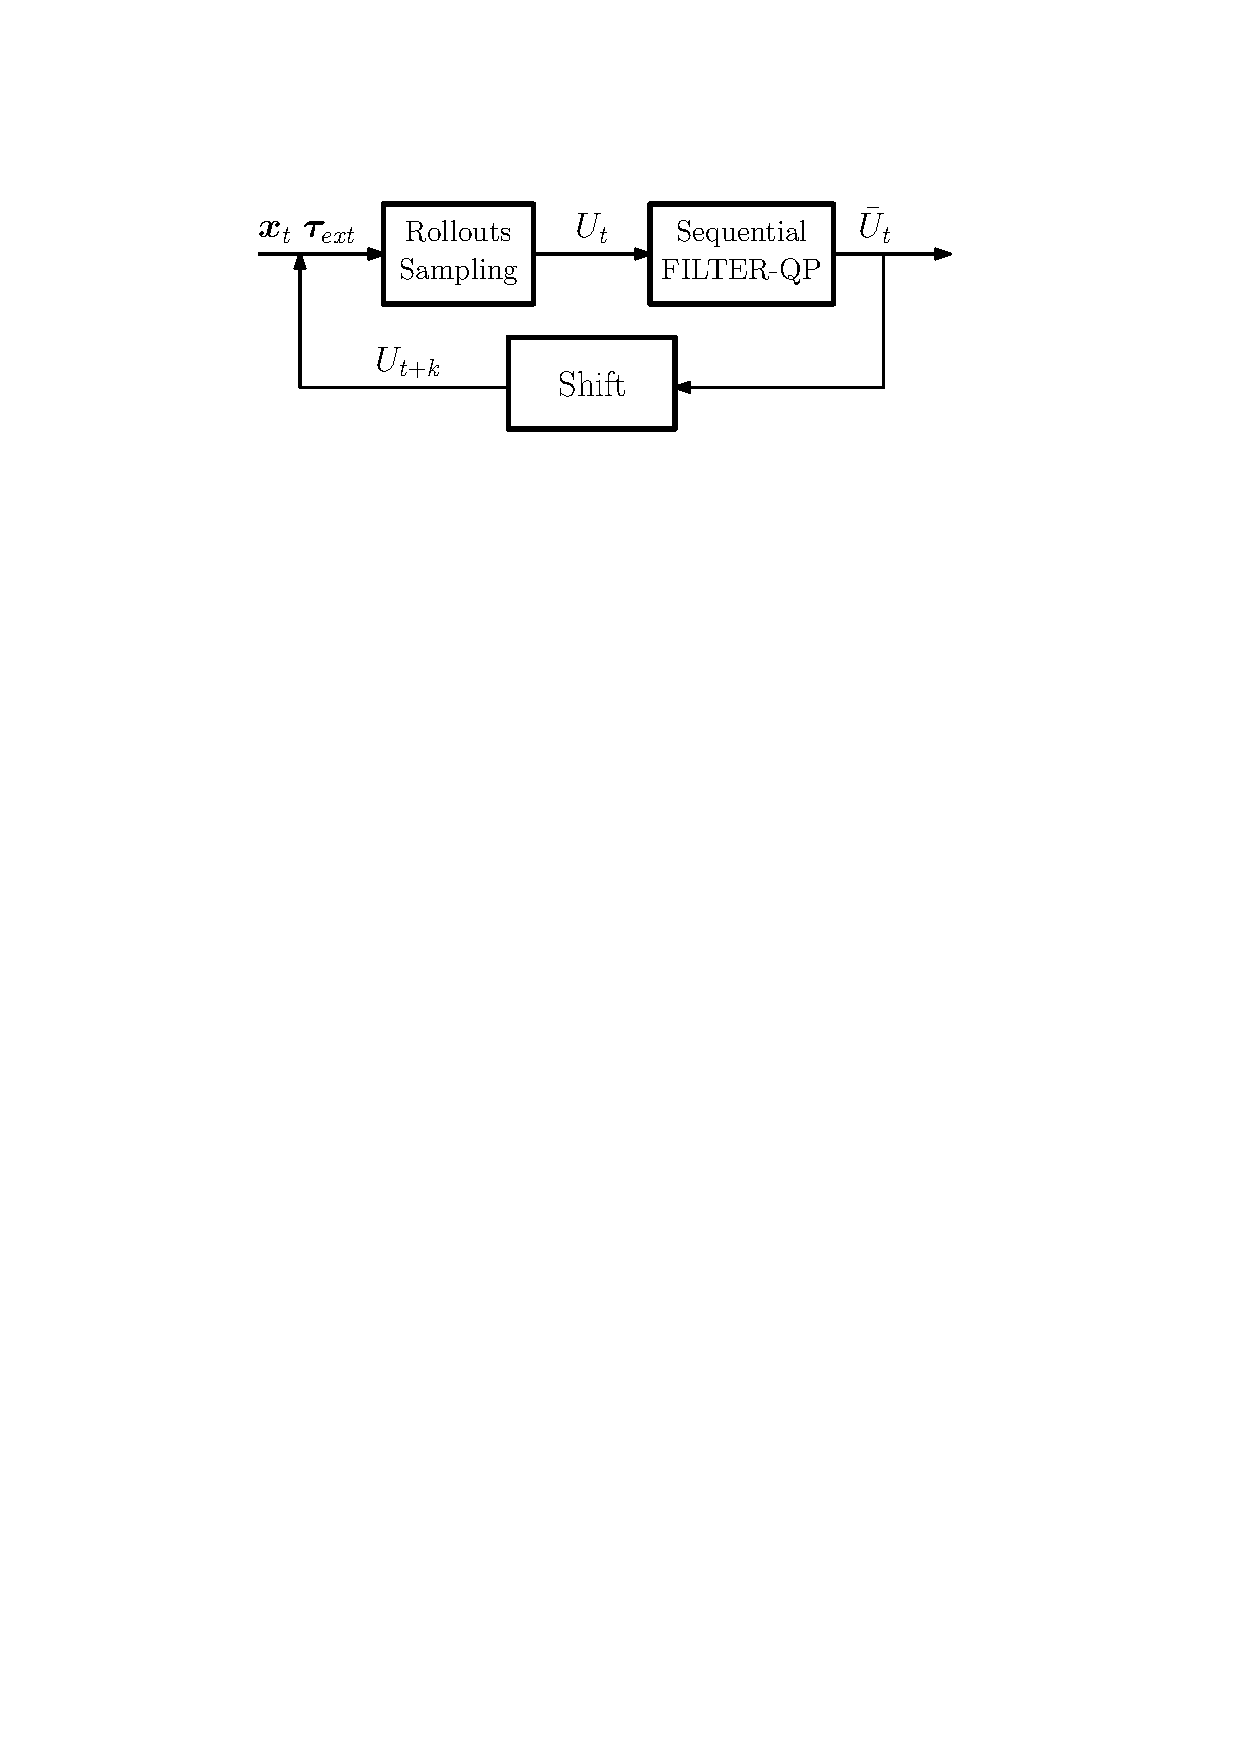
\includegraphics[width=0.8\columnwidth]{figures/schemes/stochastic_controller.pdf}
\caption{Put caption cascaded control architecture} \label{fig:cascaded_architecture}
\end{figure}

